%%%% Paramétrage du cours %%%%
\def\xxactivite{Cours}

\fichefalse \proftrue \tdfalse \courstrue

\def\xxnumchapitre{Chapitre 0 \vspace{.2cm}}
\def\xxchapitre{\hspace{.12cm} Utilisation de Python}

\def\xxcompetences{%
\textsl{%
\textbf{Savoirs et compétences :}\\
%\begin{itemize}[label=\ding{112},font=\color{bleuxp}] 
%\item Choisir un type de variable.
%\item Concevoir un algorithme utilisant une structure conditionnelle (Si), une structure itérative (while), une structure itérative (for).
%\item Concevoir une fonction.
%\item  Manipuler des listes.
%\item Instruction et expression.
%\end{itemize}
}}

\def\xxfigures{
%\includegraphics[width=\linewidth]{matlab}
%\\
%\textit{Modèle du pilote hydraulique avec pilotage interactif.}
}%figues de la page de garde

\input{\repRel/Style/pagegarde_cours}
\setlength{\columnseprule}{.1pt}

\vspace{2cm}
\pagestyle{fancy}
\thispagestyle{plain}

%%%%%%%%%%%%%%%%%%%%%%%

L'environnement de développement utilisé au lycée pour programmer en Pyhon est \texttt{Pyzo}.
\section{Installation de PYZO sur votre ordinateur personnel}
Rendez-vous sur le site \texttt{Pyzo.org} qui vous propose une fenêtre \texttt{Quickstart}.\\
L'installation se fait en quatre temps selon les éléments choisis :
\begin{enumerate}
\item Installation de l'IDE, choisir la version correspondant à votre système d'exploitation (Windows, MacOS, Linux) en 32 ou 64 bits ;
\item Installer la distribution \texttt{Anaconda} ;
\item Configurer votre shell au lancement de \texttt{Pyzo} la première fois dans la fenêtre en haut à gauche ;

\begin{center}
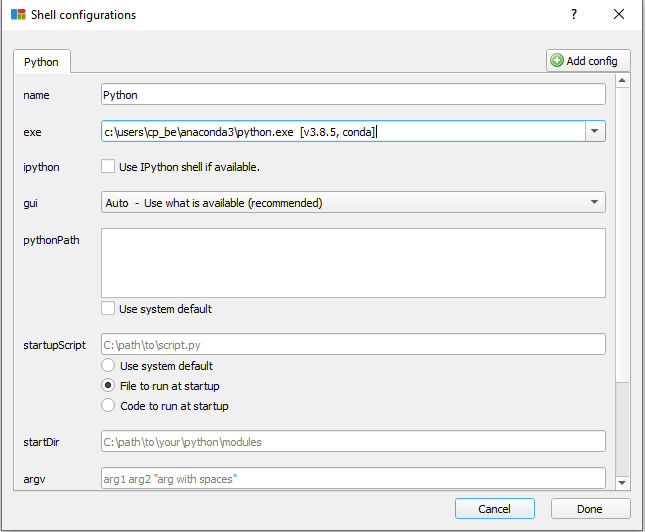
\includegraphics[scale=0.6]{Capture.png}
\end{center}

\item Les bibliothèques sont installées par défaut, l'étape 4 n'est pas utile. Sauf si vous avez dû installer une distribution plus légère.
\end{enumerate}






\section{Changement de thème de la fenêtre Pyzo}
Si l'écran blanc de la fenêtre \texttt{Pyzo} fatigue vos yeux, vous pouvez le changer :\\
setting $\backslash$ edit syntax styles... $\backslash$ \\
Vous pouvez choisir \texttt{solarized\_dark}.


\section{IDLE python}
Vous serez amené en math-info à utiliser l'IDLE Python aussi installé sur les ordinateurs du lycée.\\
Moins convivial que \texttt{Pyzo}, il permet de réaliser les mêmes travaux en utilisant les deux types de fenêtres celle du \texttt{shell} (ou \texttt{console}) et celle d'\texttt{édition}.

\begin{center}
\includegraphics[scale=0.6]{idleRunScript.png}
\end{center}

%Rendez-vous sur le site \texttt{Python.org} et choisissez votre système d'exploitation.\\
%Les deux versions \texttt{IDLE Python} et \texttt{Pyzo} peuvent être installées sur votre ordinateur sans conflit.\\
%Les bibliothèques ne sont pas installées par défaut.

L'\texttt{IDLE Python} est disponible avec toute installation de Python. Avec Pyzo, aller dans dossier contenant Pyzo ou Anaconda puis dans le répertoire \texttt{Lib\textbackslash idlelib} et lancer le programme \texttt{idle.bat}.\\
Le chemin peut être celui-ci \texttt{C:\textbackslash Users\textbackslash ...\textbackslash anaconda3\textbackslash Lib\textbackslash idlelib} par exemple.

\section{Python via des notebook : Jupyter, Capytale, Google Colab}

\subsection{Jupyter}
\texttt{Jupyter.org} est accessible par votre moteur de recherche préféré.\\
Je vous propose : \texttt{Try Jupyter} puis \texttt{JupyterLab}

\begin{center}
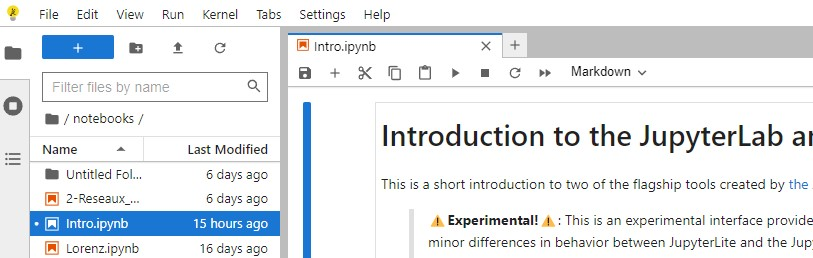
\includegraphics[scale=0.4]{jupyter.jpg}
\end{center}

Ouvrir une page vierge avec le \textbf{+} de l'onglet et sélectionner \texttt{notebook} et \texttt{Python}.


\begin{center}
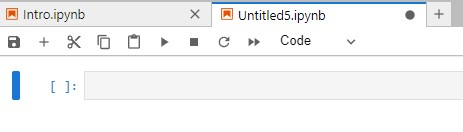
\includegraphics[scale=0.6]{jupyter2.jpg}
\end{center}

Vous pouvez écrire des lignes de codes dans la case et les exécuter avec la flèche.

\subsection{Capytale}

\texttt{Capytale} est accessible par l'ENT du lycée via \texttt{ressources numériques}. L'utilisation est la même que celle de \texttt{Jupyter}.\\
Vous y trouverez des travaux à réaliser en autonomie.

\begin{center}
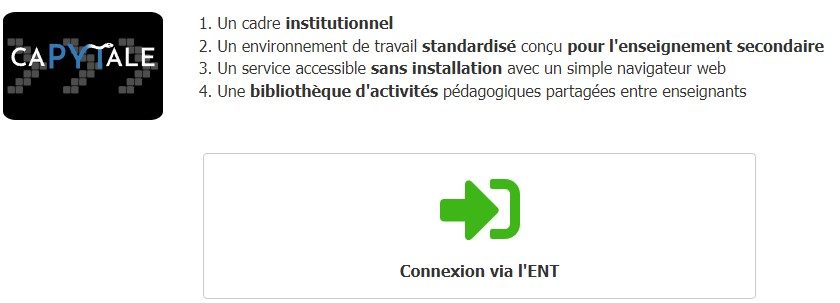
\includegraphics[scale=0.4]{capytale.jpg}
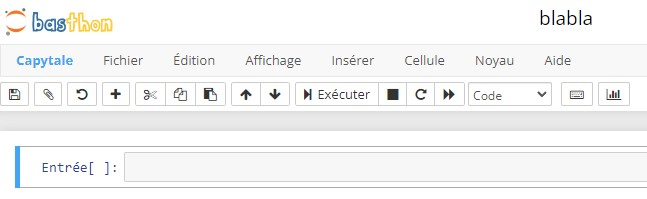
\includegraphics[scale=0.4]{capytale2.jpg}
\end{center}


\end{document}
